\documentclass[a4paper,12pt]{article}
\usepackage{graphicx}
\usepackage{float}
\usepackage[english,russian]{babel}

\title{1.1.1 Определение систематических и случайных погрешностей при измерении удельного сопротивления нихромовой проволоки}
\author{Тимур Байдюсенов Б01-302}
\date{08.09.2023}

\begin{document}
\maketitle

\section{Аннотация}
В работе размеры нихромовой проволоки измеряются с помощью линейки, штангенциркуля и микрометра, классическим методом моста постоянного тока (мост Уитстона). Сопротивление нихромовой проволоки измеряется с помощью и вольтметра и амперметра, методом моста постоянного тока. Вычисляются систематические и случайные погрешности.

\section{Теоретические сведения}
Удельное споротивление материала проволоки круглого сечения, изготовленной из однородного материала и имеющей всюду одинаковую толщину может быть определено по формуле (1):
\begin{equation}
\rho=\frac{R_}{l}\frac{\pi {d_}^2}{4}
\end{equation}
где $R_$ - сопротивление измеряемого отрезка проволоки, $l$ - его длина, $d_$ - диаметр проволоки.

Измерим $R_$ с помощью одной из схем, представленных на Рис. 1
\begin{figure}[H]
\centering
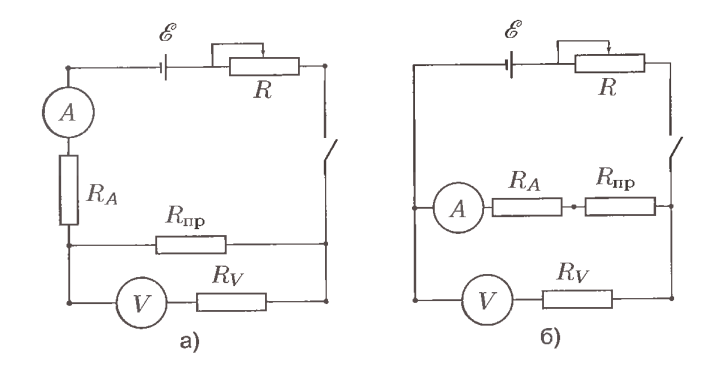
\includegraphics{схемы}
\caption{Схемы для измерения сопротивления}
\end{figure}

Схема а) Вольтметр измеряет напряжение на концах проволоки, а ампертметр измеряет ток, протекающий через вольтметр и амперметр, поэтому
\begin{equation}
R_{\mbox{пр1}}=\frac{U_a}{I_a}=R_{\mbox{пр}} \frac{R_V}{R_{\mbox{пр}}+R_V}
\end{equation}
Преобразуем формулу
\begin{equation}
R_{\mbox{пр}}=R_{\mbox{пр1}} \frac{R_V}{R_V-R_{\mbox{пр1}}}=\frac{R_{\mbox{пр1}}}{1-\frac{R_{\mbox{пр1}}}{R_V}}\approx R_{\mbox{пр1}} \left( 1+\frac{R_{\mbox{пр1}}}{R_V}\right)
\end{equation}

Схема б) Вольтметр измеряет напряжение на проволоке и амперметре, а ампертметр измеряет ток, протекающий через проволоку и амперметр, поэтому
\begin{equation}
R_{\mbox{пр2}}=\frac{U_{\mbox{б}}}{I_{\mbox{б}}} = R_{\mbox{пр}}+R_A
\end{equation}
Преобразуем формулу
\begin{equation}
R_{\mbox{пр}}=R_{\mbox{пр2}} \left( 1-\frac{R_{\mbox{А}}}{R_{\mbox{пр2}}} \right)
\end{equation}

\section{Оборудование}

\begin{table}[H]
\centering
\caption{Характеристики вольтметра}
\begin{tabular}{|c|c|}
\hline
Система & Магнитно-электрическая \\
\hline
Класс точности & 0.2 \\
\hline
Шкала & линейная, 150 делений  \\
\hline
Предел измерений & 0.6 В \\
\hline
Цена деления & 4 мВ \\
\hline
Чувствительность & 250 дел/В \\
\hline
Внутреннее сопротивление & 4 кОм \\
\hline
Погрешность при считывании со шкалы & $\pm 2$ мВ \\
\hline
Макс. погрешность & $\pm1.2$ мВ \\
\hline
\end{tabular}
\end{table}

\begin{table}[H]
\centering
\caption{Характеристики амперметра}
\begin{tabular}{|c|c|}
\hline
Система & Цифровая \\
\hline
Предел измерений & 2 A \\
\hline
Разрядность дисплея & 5 ед. \\
\hline
Внутреннее сопротивление & 1,4 Ом \\
\hline
Погрешность & $\pm (0.002x+2k)$ мА \\
\hline
\end{tabular}
\end{table}

\begin{table}[H]
\centering
\caption{Характеристики моста постоянного тока P4833}
\begin{tabular}{|c|c|}
\hline
Класс точности & 0.1 \\
\hline
Разрядность магазина сопротивлений & 5 ед. \\
\hline
Используемый диапазон измерений & $10^{-4} - 10$ Ом \\
\hline
Погрешность в использумемом диапазоне & $\pm 0.01$ Ом \\
\hline
\end{tabular}
\end{table}

Штангенциркуль: $\Delta_{\mbox{шт}} = \pm 0.05$ мм

Микрометр : $\Delta_{\mbox{мкм}} = \pm 0.005$ мм

Исходя из характеристик приборов можно заметить, что при $R_{\mbox{пр}}
\approx 5$ Ом и $R_{\mbox{A}}$ = 1.5 A, чтобы погрешность была меньше и ответ получился точнее, измерения лучше проводить с помщью схемы 1а.
Поэтому измерения будем проводить с помощью схемы 1а.

\section{Результаты измерений и обработка данных}
\subsection{Измерение диаметра проволоки}
Диаметр измерялся с помощью штангенциркуля и микрометра многократно на разных участках проволоки. Результаты представлены в таблице.
\begin{table}[H]
\label{Диаметр}
\caption{Результаты измерения диаметра проволоки}
\begin{tabular}{|c|c|c|c|c|c|c|c|c|c|c|}
\hline
$N_{\mbox{изм}}$ & 1 & 2 & 3 & 4 & 5 & 6 & 7 & 8 & 9\\
\hline
Микрометр: d, мм & 0.37 & 0.37 & 0.37 & 0.37 & 0.37 & 0.36 & 0.37 & 0.36 & 0.37 \\
\hline
Штангенциркуль: d, мм & 0.4 & 0.4 & 0.4 & 0.4 & 0.4 & 0.4 & 0.4 & 0.4 & 0.4 \\
\hline
\end{tabular}
\end{table}

\begin{table}[H]
\centering
\caption{Обработка результатов измерения диаметра}
\begin{tabular}{|c|c|c|}
\hline
 & Микрометр & Штангенциркуль \\
\hline
Средний диаметр, мм: $\overline{d}=\frac{\sum d_i}{N}$ & 0.368 & 0.4 \\
\hline
Стандартное отклонение: $\sigma_d=\sqrt{\frac{1}{N-1}\sum (d_i-\overline{d})^2}$ & 0.004&0 \\
\hline
Случайная погрешность среднего: $\sigma_{\overline{d}}=\frac{\sigma_d}{\sqrt{N}}$ & 0.001 & 0 \\
\hline
Инструментальная погрешность, мм: $\Delta$ & 0.005 & 0.05 \\
\hline
Полная погрешность: $\sigma_{\mbox{пол}}=\sqrt{\sigma_{\overline{d}}^2+\sigma_d^2}$ & 0.006 & 0.05 \\
\hline
Окончательные результаты измерения:  & 0.368 $\pm$ 0.006 & 0.4 $\pm$ 0.05 \\
\hline
\end{tabular}
\end{table}

Дальше будем использовать значение диаметра, полученное  с помощью микрометра, т.к. погрешность при использовании микрометра меньше.

Найдём площадь поперечного сечения проволоки:
\begin{equation}
S=\frac{\pi {d_}^2}{4} = \frac{\mbox{3.14} \cdot \left({\mbox{3.68} \cdot {\mbox{10}}^{\mbox{-2}}}\right)^2}{4} \approx {\mbox{1.06}} \cdot {\mbox{10}}^{\mbox{-3}} {\mbox{см}}^{\mbox{2}}
\end{equation}
Найдём величину погрешности:
\begin{equation}
\sigma_S=2\frac{\sigma_d}{d}S \approx 3.46\cdot10^{-5} {\mbox{см}}^2
\end{equation}

\subsection{Измерения сопротивления проволоки}

\begin{table}[H]
\centering
\caption{Результаты измерения напряжения и силы тока}
\begin{tabular}{|c|c|c|c|c|c|}
\hline
   \multicolumn{6}{|c|}{$l = 50 \pm 0.1$ см}\\
\hline
I, мА & 61.05 & 66.83 & 71.64 & 78.69 & 84.73\\
\hline
V, деления & 78 & 86 & 92 & 101 & 109\\
\hline
V, мВ & 312 & 344 & 368 & 404 & 436\\
\hline

I, мА & 89.69 & 96.27 & 102.83 & 108.35 & 113.63\\
\hline
V, деления & 116 & 124 & 133 & 140 & 147\\
\hline
V, мВ & 464 & 496 & 532 & 560 & 588\\
\hline
\hline

   \multicolumn{6}{|c|}{$l = 30 \pm 0.1$ см} \\
\hline
I, мА & 88.60 & 101.15 & 111.70 & 121.40 & 130.37 \\
\hline
V, деления & 68 & 77 & 85 & 92 & 99 \\
\hline
V, мВ & 272 & 308 & 340 & 368 & 396 \\
\hline

I, мА & 142.27 & 152.81 & 162.92 & 172.77 & 186.26  \\
\hline
V, деления & 109 & 117 & 125 & 132 & 142 \\
\hline
V, мВ & 436 & 468 & 500 & 528 & 568 \\
\hline
\hline

   \multicolumn{6}{|c|}{$l = 20 \pm 0.1$ см} \\
I, мА & 109.57 & 122.63 & 135.26 & 149.23 & 164.52  \\
\hline
V, деления & 55 & 62 & 68 & 76 & 83 \\
\hline
V, мВ & 220 & 248 & 272 & 304 & 332 \\
\hline

I, мА & 180.13 & 192.03 & 212.81 & 234.57 & 253.83 \\
\hline
V, деления & 92 & 97 & 108 & 119 & 128 \\
\hline
V, мВ & 368 & 388 & 432 & 476 & 512  \\
\hline

\end{tabular}
\label{ампвол}
\end{table}

\begin{figure}[H]
\centering
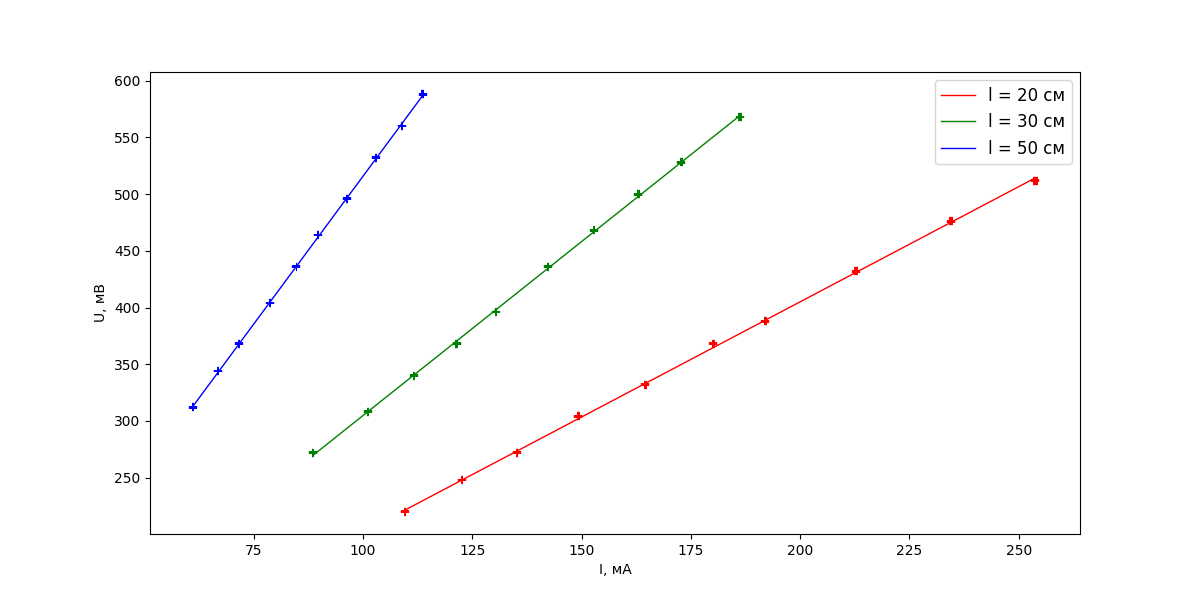
\includegraphics[scale = 0.5]{графики}
\caption{Вольт-амперная характеристика}
\end{figure}

\begin{table}[H]
\centering
\caption{Результаты измерения сопротивления проволок с помощью амперметра и вольтметра}
\begin{tabular}{|c|c|c|c|c|c|}
\hline
$l, $см & $R_{\mbox{ср}}$, Ом & $\sigma_{R_{\mbox{ср}}}^{\mbox{случ}}$, Ом & $\sigma_{R_{\mbox{ср}}}^{\mbox{сист}}$, Ом & $\sigma_{R_{\mbox{ср}}}$, Ом & $R_{\mbox{пр}}$, Ом\\
\hline
20 & 2.02 & 0.0003 & 0.004 & 0.004 & 2.021\\
\hline
30 & 3.06 & 0.0007 & 0.007 & 0.007 & 3.062\\
\hline
50 & 5.16 & 0.0010 & 0.011 & 0.011 & 5.167\\
\hline
\end{tabular}
\end{table}

Вычислим $\sigma_{R_{\mbox{ср}}}^{\mbox{случ}}$ по формуле:

\begin{equation}
\sigma_{R_{\mbox{ср}}}^{\mbox{случ}}=\frac{\sqrt{\sum_{i = 1}^{10}{\frac{V{\mbox{i}}^2}{I{\mbox{i}}^2}}-R_{\mbox{ср}}^2}}{\sqrt{10} \cdot \sqrt{9}} \cdot t_{\mbox{p}}
\end{equation}

Возможную систематическую погрешность $R_{\mbox{ср}}$ оцениваем по формуле:

\begin{equation}
\frac{\sigma_{R_{\mbox{ср}}}^{\mbox{сист}}}{R_{\mbox{ср}}}=\sqrt{\left( \frac{\sigma_V}{V} \right)^2+\left( \frac{\sigma_I}{I} \right)^2}
\end{equation}

\begin{table}[H]
\centering
\caption{Результаты измерения сопротивления проволок с помощью моста P4833}
\begin{tabular}{|c|c|}
\hline
$l, $см & $R_0$, Ом \\
\hline
20 & 2.04 $\pm$ 0.01 \\
\hline
30 & 3.07 $\pm$ 0.01 \\
\hline
50 & 5.19 $\pm$ 0.01 \\
\hline
\end{tabular}
\end{table}

В на графике и в таблицах 6, 7 и 8 представлены результаты измерения сопротивления проволок с помощью вольтметра и амперметра, моста постоянного тока P4833. Вычисление R производилось по формуле (3).

Можно заметить, что систематические ошибки на порядок больше случайных, поэтому  результаты измерений очень близки к настоящим значениям.

\subsection{Измерение удельного сопротивления проволоки}

Найдем удельное сопротивление проволоки по формуле:
\begin{equation}
\rho = R\frac{S}{l}
\end{equation}
\begin{equation}
\sigma_{\rho} = \sqrt{\left( \frac{\sigma_R}{R} \right)^2+\left( 2 \cdot \frac{\sigma_d}{d} \right)^2+\left(\frac{\sigma_l}{l} \right)^2}
\end{equation}
Значения удельного сопротивления для каждой из длин представлены в таблице 9

\begin{table}[H]
\centering
\caption{Результаты $\rho$ для каждой из длин проволок}
\begin{tabular}{|c|c|c|}
\hline
$l$, см & $\rho$, $10^{-6}$ Ом $\cdot$м &$\sigma_{\rho}$, $10^{-8}$Ом$\cdot$м \\
\hline
20 & 1.07 & 3.6 \\
\hline
30 & 1.08 & 3.5 \\
\hline
50 & 1.10 & 3.5 \\
\hline
\end{tabular}
\end{table}

Окончательно: $\rho = (1.08 \pm 0.04)\cdot 10^{-6}$ Ом$\cdot$м.

\section{Вывод}
Полученное значение удельного сопротивления сравниваем с табличными значениями. В справочнике (Физические величины. М.:Энергоиздат, 1991. С. 444) для удельного сопротивления нихрома при 20 \textdegree C, значения в зависимости от массового содержания компонент сплава меняются от 1.12$\cdot10^{-4}$ Ом$\cdot$см до 0.97$\cdot10^{-4}$ Ом$\cdot$см. Наиболее близкое значение к получившемуся в работе 1.06$\cdot10^{-4}$ Ом$\cdot$см.
Мои значения совпали в пределах погрешности: $\rho = (1.08 \pm 0.05)\cdot 10^{-6}$ Ом$\cdot$м.

\end{document}
